\chapter{Metodologia}\label{metodologia}
Com o objetivo de apresentar os aspectos metodológicos e teóricos desta tese, optou-se por organizar este capítulo em seções que se inter-relacionam para fornecer a descrição dos modelos, das detecção de bordas e das abordagens para a fusão das evidências de bordas. 
\section{Modelagem estatística para dados PolSAR}\label{cap_model_estatistica}
Os sistemas PolSAR transmitem pulsos de micro-ondas polarizados ortogonalmente e medem componentes ortogonais do sinal recebido. Para cada pixel, a medida resulta em uma matriz de coeficientes de espalhamento. Esses coeficientes são números complexos que descrevem no sistema SAR a transformação do campo eletromagnético transmitido para o campo eletromagnético recebido.

A transformação pode ser representada como
\begin{equation*}
 \left[
\begin{array}{c}
	E_\text{h}^\text{r}   \\
	E_\text{v}^\text{r}    \\
\end{array}
\right]
 = \frac{e^{\hat{\imath} \text{kd}}}{\text{d}}\left[
\begin{array}{cc}
	S_{\text{hh}}   & S_{\text{hv}}   \\
	S_{\text{vh}}   & S_{\text{vv}}   \\
\end{array}
\right]
 \left[
\begin{array}{c}
	E_\text{h}^\text{t}   \\
	E_\text{v}^\text{t}   \\
\end{array}
\right],
\end{equation*}
onde k denota o número de onda, $\hat{\imath}$ é um número complexo e d é a distância entre o radar e o alvo. No campo eletromagnético com componentes $E_\text{i}^\text{j}$, o índice subscrito denota polarização horizontal (h) ou vertical (v), e o índice sobrescrito indica a onda recebida (r) ou transmitida (t). 

A matriz de espalhamento complexa $\mathbf{S}$ é definida por
\begin{equation}\label{matriz_de_espalhamento}
\mathbf{S} = \left[
\begin{array}{cc}
	S_\text{hh}   & S_\text{hv}   \\
	S_\text{vh}   & S_\text{vv}   \\
\end{array}
\right],
\end{equation}\index{Matriz de Espalhamento}
onde as entradas da matriz $S_\text{i,j}$ são os coeficientes de espalhamento complexo, tal que os índices i e j são associados ao  recebimento e a transmissão das ondas, por exemplo, o coeficiente de espalhamento $S_\text{hv}$ está associado a onda transmitida na direção vertical (v) e recebida na direção horizontal (h).

Definindo a diagonal principal da matriz de espalhamento por co-polarização pois relaciona a polarização das ondas transmitidas e recebidas nas mesmas direções, e a os elementos da diagonal secundária da matriz de espalhamento por polarização cruzada relacionando os estados de polarizações ortogonais.
% ver~\citep{lp}.
 
%A matriz $\mathbf{S}$ depende da definição do sistema de coordenadas, se a antena transmissora e receptora de sinal estão localizadas na mesma posição as medidas são mono-estáticas, e consideramos o sistema de coordenada BSA - \textit{Back Scattering Alignment}, assim o sistema de coordenadas da transmissão e recepção de sinal são coincidentes.   
 
A potência total espalhada no caso de um sistema de radar polarimétrico é o chamado \textit{Span}, sendo definido no caso geral como,
\begin{equation}\label{span_geral}
\mathit{Span}(\mathbf{S}) = \traco(\mathbf{S}\mathbf{S}^H)=|S_\text{hh}|^2+|S_\text{hv}|^2+|S_\text{vh}|^2+|S_\text{vv}|^2,
\end{equation}\index{Span}
onde o operador $\traco(\cdot)$ é o traço de uma matriz.


\subsection{Matriz de coerência polarimétrica de Pauli ($\mathbf{T}_4$) e matriz de covariância lexicográfica ($\mathbf{C}_4$)}
A matriz de espalhamento $\mathbf{S}$ pode ser representada pela construção do vetor,
\begin{equation}\label{def_vet_espalhamento_4d}
\mathbf{k}=\frac{1}{2}\left[\traco(\mathbf{S}\Psi_1)\quad\traco(\mathbf{S}\Psi_2)\quad \traco(\mathbf{S}\Psi_3)\quad \traco(\mathbf{S}\Psi_4)\right]^T,
\end{equation}
onde $\{\Psi_i\}_{i=1}^4$ é uma base para o espaço das matrizes hermitianas $2\times 2$.

Diferentes bases para o mesmo espaço das matrizes podem ser definidas, vamos escolher duas bases, a primeira chamada de  base de Pauli,
\begin{equation}\label{base_de_pauli_4d}
\{\Psi_P\} = \left\{
\sqrt{2}\left[\begin{array}{cc}
	1  & 0  \\
	0  & 1 \\
\end{array}\right],
\sqrt{2}\left[\begin{array}{cc}
	1  & 0  \\
	0  & -1  \\
\end{array}\right],
\sqrt{2}\left[\begin{array}{cc}
	0  & 1  \\
	1  & 0  \\
\end{array}\right],
\sqrt{2}\left[\begin{array}{cc}
	0       & -i  \\
	i  & 0  \\
\end{array}\right]
\right\},
\end{equation}\index{Base de Pauli de dimensão 4}
e a segunda chamada de base lexicográfica,
\begin{equation}\label{base_lexicografica_4d}
\{\Psi_L\} = \left\{
2\left[\begin{array}{cc}
	1  & 0  \\
	0  & 0 \\
\end{array}\right],
2\left[\begin{array}{cc}
	0  & 1  \\
	0  & 0  \\
\end{array}\right],
2\left[\begin{array}{cc}
	0  & 0  \\
	1  & 0 \\
\end{array}\right],
2\left[\begin{array}{cc}
	0  & 0  \\
	0  & 1  \\
\end{array}\right]
\right\}.
\end{equation}\index{Base Lexicográfica de dimensão 4}

Sendo o vetor \eqref{def_vet_espalhamento_4d}, e usando a base \eqref{base_de_pauli_4d} representamos a matriz de espalhamento pelo vetor característico de Pauli $4$-D,
\begin{equation}\label{vetor_pauli_4d}
\mathbf{k}= \frac{1}{\sqrt{2}}\left[
	\begin{array}{cccc}
	S_\text{hh} + S_\text{vv}& S_\text{hh} - S_\text{vv}& S_\text{hv} + S_\text{vh} &i (S_\text{hv} - S_\text{vh})   \\
\end{array}\right]^T=\frac{1}{\sqrt{2}}[k_1\quad k_2\quad k_3\quad k_4],
\end{equation}
e usando a base \eqref{base_lexicografica_4d} representamos a matriz de espalhamento pelo vetor característico lexicográfico $4$-D, 
\begin{equation}\label{vetor_lexicografico_4d}
\mathbf{\Omega}= \left[
	\begin{array}{cccc}
	S_\text{hh}& S_\text{hv} &S_\text{hv}& S_\text{vv}   \\
\end{array}\right]^T=[\Omega_1\quad \Omega_2\quad \Omega_3\quad \Omega_4].
\end{equation}

A matriz de espalhamento pode ser relacionada com os vetores \eqref{vetor_pauli_4d} e \eqref{vetor_lexicografico_4d} da seguinte maneira,
\begin{equation}\label{mat_esp_rel_pauli_lex}
\mathbf{S} = \left[
\begin{array}{cc}
	S_\text{hh}   & S_\text{hv}   \\
	S_\text{vh}   & S_\text{vv}   \\
\end{array}
\right]=
\left[
\begin{array}{cc}
	\Omega_1   & \Omega_2   \\
	\Omega_3   & \Omega_4   \\
\end{array}
\right]=\frac{1}{\sqrt{2}}
\left[
\begin{array}{cc}
	 k_1+k_2  & k_3-ik_4   \\
	 k_3+ik_4 & k_1-k_2   \\
\end{array}
\right]
\end{equation}

As constantes $2$ e $\sqrt{2}$ nas bases \eqref{base_de_pauli_4d} e \eqref{base_lexicografica_4d} ajustam a norma dos vetores de espalhamento para serem iguais, independente da escolha das bases. O produto interno escolhido é o padrão para o espaço vetorial dos vetores complexos de dimensão 4, isto é, se $\mathbf{u}$ e $\mathbf{v}$ são vetores complexos, o produto interno é $\mathbf{u}^\text{H}\mathbf{v}$.

Podemos assim garantir a invariância do 
\begin{equation}\label{span_invariante}
\begin{array}{ccccc}
\mathit{Span}(\mathbf{S}) &=&\traco(\mathbf{S}\mathbf{S}^\text{H})&=&|S_\text{hh}|^2+|S_\text{hv}|^2+|S_\text{vh}|^2+|S_\text{vv}|^2  \\
	   &=&  \mathbf{k}^\text{H}\mathbf{k}&=&|\mathbf{k}|^2\\
	   &=&\mathbf{\Omega}^\text{H}\mathbf{\Omega} &=&|\mathbf{\Omega}|^2.\\
\end{array}
\end{equation}

A matriz unitária $\mathbf{U}_4$ é definida como a representação matricial da transformação linear que aplica o vetor na base lexicográfica em um vetor na base de Pauli. Podemos gerar a  matriz unitária colocando nas linhas da matriz os elementos da base de Pauli, portanto
\begin{equation}\label{matriz_unit_su4}
\mathbf{U}_4=	\frac{1}{\sqrt{2}}	
\left[
\begin{array}{rrrr}
	1   & 0 & 0 & 1  \\
	1   & 0 & 0 & -1  \\
	0   & 1 & 1 & 0  \\
	0   & i & -i &0   \\
\end{array}
\right].
\end{equation}

A transformação linear $\mathbf{k}=\mathbf{U}_4\mathbf{\Omega}$, representada na forma matricial,
\begin{equation}\label{trans_matriz_unit_su4}
\frac{1}{\sqrt{2}}\left[
\begin{array}{c}
	  S_\text{hh} +  S_\text{vv}\\  
	  S_\text{hh} -  S_\text{vv}\\
	  S_\text{hv} +  S_\text{vh} \\
        i(S_\text{hv} -  S_\text{vh}) \\
\end{array}
\right]=\frac{1}{\sqrt{2}}	
\left[
\begin{array}{rrrr}
	1   & 0 & 0 & 1  \\
	1   & 0 & 0 & -1  \\
	0   & 1 & 1 & 0  \\
	0   & i & -i &0   \\
\end{array}
\right]
\left[
\begin{array}{c}
	S_\text{hh} \\  
	S_\text{hv} \\
	S_\text{vh} \\
	S_\text{vv} \\
\end{array}
\right],
\end{equation}
foi definida para demonstrar a transformação similar entre a matriz de coerência, e a matriz de covariância definidas a seguir.  

A matriz de coerência polarimétrica de Pauli é definida por, 
\begin{equation}\label{matriz_polar_pauli}
	\mathbf{T}_4=\mathbf{k}\mathbf{k}^\text{H}=	
\left[
\begin{array}{rrrr}
	|k_1|^2       & k_1\bar{k}_2  & k_1\bar{k}_3  & k_1\bar{k}_4  \\
	k_2\bar{k}_1  & |k_2|^2       & k_2\bar{k}_3  & k_2\bar{k}_4  \\
	k_3\bar{k}_1  & k_3\bar{k}_2  &    |k_3|^2    & k_3\bar{k}_4  \\
	k_4\bar{k}_1  & k_4\bar{k}_2  & k_4\bar{k}_3  & |k_4|^2   \\
\end{array}
\right],
\end{equation}\index{Matriz polarimétrica de Pauli $4\times 4$}
e a matriz de covariância lexicográfica
\begin{equation}\label{matriz_covar_lexic}
	\mathbf{C}_4=\mathbf{\Omega}\mathbf{\Omega}^\text{H}=	
\left[
\begin{array}{rrrr}
	|\Omega_1|^2       & \Omega_1\bar{\Omega}_2  & \Omega_1\bar{\Omega}_3  & \Omega_1\bar{\Omega}_4  \\
	\Omega_2\bar{\Omega}_1  & |\Omega_2|^2       & \Omega_2\bar{\Omega}_3  & \omega_2\bar{\Omega}_4  \\
	\Omega_3\bar{\Omega}_1  & \Omega_3\bar{\Omega}_2  &    |\Omega_3|^2    & \Omega_3\bar{\Omega}_4  \\
	\Omega_4\bar{\Omega}_1  & \Omega_4\bar{\Omega}_2  & \Omega_4\bar{\Omega}_3  & |\Omega_4|^2   \\
\end{array}
\right].
\end{equation}\index{Matriz de covariância lexicográfica $4\times 4$}

As matrizes de coerência polarimétrica de Pauli e covariância lexicográfica são relacionadas usando as definições e a propriedade \eqref{trans_matriz_unit_su4}, assim teremos
\begin{equation}\nonumber
\begin{array}{rcccr}
	\mathbf{T}_4&=&\mathbf{k}\mathbf{k}^\text{H}&=&\mathbf{U}_4\mathbf{\Omega}(\mathbf{U_4\Omega})^H	\\
	   &=&\mathbf{U_4\Omega}\mathbf{\Omega}^H\mathbf{U_4}^H&=&\mathbf{U_4}\mathbf{C}_4\mathbf{U_4}^H	\\
\end{array}
\end{equation}
então, a relação de similaridade entre as matrizes é,
\begin{equation}\label{matriz_simil_t4_c4}
\begin{array}{rrr}
	 \mathbf{T}_4  &=&\mathbf{U_4}\mathbf{C}_4\mathbf{U_4}^\text{H}\\
\end{array}
\end{equation}
lembrando que $\mathbf{U_4}$ é unitária, e o traço é a soma dos autovalores de uma matriz, concluímos
\begin{equation}\label{traco_t4_c4}
\begin{array}{rrrrr}
	\traco({\mathbf{T}_4})  &=&\traco({\mathbf{C}_4})&=&\mathit{Span}\mathbf{(S)}.\\
\end{array}
\end{equation}
\subsection{Matriz de coerência polarimétrica de Pauli ($\mathbf{T}_3$) e matriz de covariância lexicográfica ($\mathbf{C}_3$)}
Podemos entender as interações das ondas eletromagnéticas em alvos naturais sob a ótica do teorema da reciprocidade, o qual considera o meio reciproco. De uma maneira geral as propriedades de transmissão e recebimento de uma antena são idênticos, e mono-estáticos, ou seja, consideramos o sistema de coordenada BSA - \textit{Back Scattering Alignment} . Em meio reciproco podemos definir a igualdade dos termos de polarização cruzada $S_\text{hv}=S_\text{vh}$. Veja \citet{lp}. 

A matriz de espalhamento $\mathbf{S}$ pode ser representada pela construção do vetor,
\begin{equation}\label{def_vet_espalhamento_3d}
\mathbf{k}=\frac{1}{2}\left[\traco(S\Psi_1)\quad\traco(S\Psi_2)\quad \traco(S\Psi_3)\right]^T,
\end{equation}
onde $\{\Psi_i\}_{i=1}^3$ é uma base para o espaço das matrizes hermitianas $2\times 2$.

Diferentes bases para o mesmo espaço das matrizes podem ser definidas, vamos escolher duas bases, a primeira chamada de  base de Pauli,
\begin{equation}\label{base_de_pauli_3d}
\{\Psi_P\} = \left\{
\sqrt{2}\left[\begin{array}{cc}
	1  & 0  \\
	0  & 1 \\
\end{array}\right],
\sqrt{2}\left[\begin{array}{cc}
	1  & 0  \\
	0  & -1  \\
\end{array}\right],
\sqrt{2}\left[\begin{array}{cc}
	0  & 1  \\
	1  & 0  \\
\end{array}\right]
\right\},
\end{equation}\index{Base de Pauli de dimensão 3}
e a segunda chamada de base lexicográfica
\begin{equation}\label{base_lexicografica_3d}
\{\Psi_L\} = \left\{
2\left[\begin{array}{cc}
	1  & 0  \\
	0  & 0 \\
\end{array}\right],
2\sqrt{2}\left[\begin{array}{cc}
	0  & 1  \\
	0  & 0  \\
\end{array}\right],
2\left[\begin{array}{cc}
	0  & 0  \\
	0  & 1  \\
\end{array}\right]
\right\}.
\end{equation}\index{Base lexicográfica de dimensão 3}

Sendo o vetor \eqref{def_vet_espalhamento_3d}, e usando a base \eqref{base_de_pauli_3d} representamos a matriz de espalhamento pelo vetor característico de Pauli $3$-D,
\begin{equation}\label{vetor_pauli_3d}
\mathbf{k}= \frac{1}{\sqrt{2}}\left[
	\begin{array}{ccc}
	S_\text{hh} + S_\text{vv} & S_\text{hh} - S_\text{vv}& 2S_\text{hv}   \\
\end{array}\right]^T=\frac{1}{\sqrt{2}}[k_1\quad k_2\quad k_3],
\end{equation}
e usando a base \eqref{base_lexicografica_3d} representamos a matriz de espalhamento pelo vetor característico lexicográfico $3$-D,  
\begin{equation}\label{vetor_lexicografico_3d}
\mathbf{\Omega}= \frac{1}{\sqrt{2}}\left[
	\begin{array}{ccc}
	S_\text{hh}& S_\text{hv}& S_\text{vv}   \\
\end{array}\right]^T=[\Omega_1\quad \Omega_2\quad \Omega_3].
\end{equation}

As constantes $2$ e $\sqrt{2}$ nas bases \eqref{base_de_pauli_3d} e \eqref{base_lexicografica_3d} servem para manter a norma dos vetores de espalhamento iguais, independente da escolha das bases. O produto interno escolhido é o padrão para o espaço vetorial dos vetores complexos de dimensão 3, isto é, se $\mathbf{u}$ e $\mathbf{v}$ são vetores complexos, o produto interno é $\mathbf{u}^\text{H}\mathbf{v}$.

Podemos assim garantir a invariância da potencia total,
\begin{equation}\label{span_invariante_3d}
\begin{array}{ccccc}
\mathit{Span}(\mathbf{S}) &=&  \traco(\mathbf{SS}^\text{H})&=&|S_{hh}|^2+2|S_{hv}|^2+|S_{vv}|^2  \\
	   &=&  \mathbf{k}^\text{H}\mathbf{k}&=&|\mathbf{k}|^2\\
	   &=&  \mathbf{\Omega}^\text{H}\mathbf{\Omega}&=&|\mathbf{\Omega}|^2\\
\end{array}
\end{equation}

A matriz unitária $\mathbf{U}_3$ é definida como a representação matricial da transformação linear que aplica o vetor na base lexicográfica em um vetor na base de Pauli. Podemos gerar a  matriz unitária colocando nas linhas da matriz os elementos da base de Pauli, portanto
\begin{equation}\label{matriz_unit_su3}
\mathbf{U}_3=\frac{1}{\sqrt{2}}	
\left[
\begin{array}{rrr}
	1   & 0 & 1  \\
	1   & 0 & -1  \\
	0   & \sqrt{2} &  0  \\
\end{array}
\right].
\end{equation}

A transformação linear $\mathbf{k}=\mathbf{U}_3\mathbf{\Omega}$, representado na forma matricial,
\begin{equation}\label{trans_matriz_unit_su3}
\frac{1}{\sqrt{2}}\left[
\begin{array}{c}
	  S_\text{hh} +  S_\text{vv}\\  
	  S_\text{hh} -  S_\text{vv}\\
	  2  S_\text{hv} \\
\end{array}
\right]=\frac{1}{\sqrt{2}}	
\left[
\begin{array}{rrr}
	1   & 0 & 1  \\
	1   & 0 & -1  \\
	0   & 2 &  0  \\
\end{array}
\right]
\left[
\begin{array}{c}
	S_\text{hh} \\  
	S_\text{hv} \\
	S_\text{vv}\\
\end{array}
\right]
\end{equation}
foi definida para demonstrar a transformação similar entre a matriz de coerência, e a matriz de covariância definidas a seguir.

A matriz de coerência polarimétrica de Pauli é definida por,
\begin{equation}\label{matriz_polar_pauli_3}
	\mathbf{T}_3=\mathbf{k}\mathbf{k}^\text{H}=	
\left[
\begin{array}{rrr}
	|k_1|^2       & k_1\bar{k}_2  & k_1\bar{k}_3  \\
	k_2\bar{k}_1  & |k_2|^2       & k_2\bar{k}_3  \\
	k_3\bar{k}_1  & k_3\bar{k}_2  &    |k_3|^2    \\
\end{array}
\right],
\end{equation}\index{Matriz polarimétrica de Pauli $3\times 3$}
e a matriz de covariância lexicográfica
\begin{equation}\label{matriz_covar_lexic_3}
	\mathbf{C}_3=\mathbf{\Omega}\mathbf{\Omega}^\text{H}=	
\left[
\begin{array}{rrr}
	|\Omega_1|^2       & \Omega_1\bar{\Omega}_2  & \Omega_1\bar{\Omega}_3   \\
	\Omega_2\bar{\Omega}_1  & |\Omega_2|^2       & \Omega_2\bar{\Omega}_3  \\
	\Omega_3\bar{\Omega}_1  & \Omega_3\bar{\Omega}_2  &    |\Omega_3|^2      \\
\end{array}
\right].
\end{equation}\index{Matriz de covariância polarimétrica $3\times 3$}

As matrizes de coerência polarimétrica de Pauli e covariância lexicográfica são relacionadas usando as definições e a propriedade \eqref{trans_matriz_unit_su4}, assim teremos
\begin{equation}\nonumber
\begin{array}{rrrrr}
	\mathbf{T}_3&=&\mathbf{k}\mathbf{k}^\text{H}&=&\mathbf{U_3\Omega}(\mathbf{U_3\Omega})^\text{H}	\\
	   &=&\mathbf{U_3\Omega}\mathbf{\Omega}^\text{H}\mathbf{U_3}^\text{H}&=&\mathbf{U_3}\mathbf{C}_3\mathbf{U_3}^\text{H}\\
\end{array},
\end{equation}
então, a relação de similaridade entre as matrizes é,
\begin{equation}\label{matriz_simil_t3_c3}
\begin{array}{rrr}
	 \mathbf{T}_3  &=&\mathbf{U_3}\mathbf{C}_3\mathbf{U_3}^\text{H}\\
\end{array},
\end{equation}
lembrando que $\mathbf{U_3}$ é unitária, e o traço é a soma dos autovalores de uma matriz, concluímos
\begin{equation}\label{traco_t3_c3}
\begin{array}{rrrrr}
	\traco({\mathbf{T}_3})  &=&\traco({\mathbf{C}_3})&=&\mathit{Span}\mathbf{(S)}.\\
\end{array}
\end{equation}

Portanto podemos afirmar, se
\begin{equation}\label{vetor_3d} 
\mathbf{s} = \left[
\begin{array}{c}
	S_\text{hh}      \\
        \sqrt{2}S_\text{hv}     \\
	S_\text{vv}      \\
\end{array}
\right],
\end{equation}
a potência total espalhada no caso de um sistema de radar polarimétrico em meio recíproco pode ser definido por
\begin{equation}\label{span_geral}
\mathit{Span} = \traco(\mathbf{SS}^\text{H})=|S_\text{hh}|^2+2|S_\text{hv}|^2+|S_\text{vv}|^2.
\end{equation}

\subsection{Estatística do Ruído \textit{Speckle} no processo de única visada}\index{O ruído \textit{Speckle}}
As imagens SAR e PolSAR possuem um tipo de ruído multiplicativo chamado \textit{speckle}, conhecido por causar variação de intensidade pixel a pixel, imprimindo um aspecto granular as imagens.  

O \textit{speckle} dificulta a interpretação e análise das imagens reduzindo a efetividade da segmentação, classificação, ou detecção de mudanças de características das imagens SAR e PolSAR. O entendimento do comportamento estatístico do \textit{speckle} é essencial para extrair boas informações das imagens e propor algoritmos efetivos para tratar esse tipo de ruído. 

Neste trabalho usaremos as características do ruído \textit{speckle} para auxiliar na detecção de borda, em oposição a trabalhos que tentam mitigar o efeito do ruído.
  
A formação do \textit{speckle} surge quando o radar ilumina uma superfície rugosa, como florestas, plantações, áreas urbanas, e etc, então o sinal de retorno consiste em ondas refletidas com muitos elementos de espalhamentos. Os elementos de espalhamento têm geometrias complexas e distribuições aleatórias, tornando a modelagem estatística uma tarefa indispensável e desafiadora. Podemos considerar três tipos de processos de espalhamento da onda em alvos (elementos de espalhamento). A dispersão de superfície, a dispersão de volume, e o espalhamento de volume-superfície. O primeiro é o espalhamento que acontece quando a onda eletromagnética atravessa uma mudança de meio de propagação. O segundo, consiste no espalhamento que acontece na profundidade de um meio, por exemplo, o espalhamento no interior de uma floresta. E por último, o espalhamento volume-superfície, que consiste em a onda atingir outra troca de meio de propagação, por exemplo o solo de uma floresta.
 
 As distância entre os elementos de espalhamento e o recebimento no radar varia devido a natureza randômica da disposição desse elemento. A onda recebida de cada elemento espalhador embora coerente em frequência não são coerentes em fase. O sinal é forte se as ondas são construtivas, ou seja em fase, e fraco se a ondas não estão em fase.
 
Podemos escrever um sinal complexo da seguinte forma.
\begin{equation}\label{eq:speckle_soma}
\sum_{i=1}^{M}(x_i+\hat{\jmath} y_i)=\sum_{i=1}^{M}x_i+\hat{\jmath}\sum_{i=1}^{M} y_i=x+\hat{\jmath} y=r\exp(\hat{\jmath}\theta),
\end{equation}
onde,~$x_i+\hat{\jmath} y_i$ é o retorno do espalhamento para cada elemento $i$, se existem $M$ elementos espalhadores então $x+\hat{\jmath}y$ é soma destes elementos, e $r\exp(\hat{\jmath}\theta)$ é a decomposição de Euler para o número complexo $x+\hat{\jmath}y$.
\subsubsection{Modelo de Rayleigh para o \textit{speckle}}
Definir um modelo para o \textit{speckle} é muito importante na tarefa de obter informação de imagens SAR e PolSAR. Com esse objetivo, podemos determinar as seguintes condições para a modelagem:
\begin{itemize}
\item Um número grande de espalhadores em uma região (célula de resolução) considerada um meio homogêneo.
\item A distância de alcançe é muito maior que o comprimento de onda do radar.
\item A superfície tem maior rugosidade na escala do comprimento de onda de um radar.
\end{itemize}

O \textit{speckle} totalmente desenvolvido é definido utilizando o vetor soma \eqref{eq:speckle_soma} para os retornos dos espalhamentos de alvos de forma que a sua fase seja distribuída uniformemente no intervalo $(-\pi,\pi)$. 

O teorema do limite central para o \textit{speckle} totalmente desenvolvido garante que as componentes $x$ e $y$ sejam gaussianas independentes e identicamente distribuídas com média zero e variância $\frac{\sigma^2}{2}$. Podemos representar a sua função densidade de probabilidade conjunta por,
\begin{equation}\label{eq:pdf_gaussiana_xy}
\begin{split}
  f_{XY}(x,y;\sigma^2)&=f_X(x;\sigma^2)f_Y(y;\sigma^2)\\
  &=\frac{1}{\sqrt{\pi}\sigma}\exp\left(-\frac{x^2}{\sigma^2}\right)\frac{1}{\sqrt{\pi}\sigma}\exp\left(-\frac{y^2}{\sigma^2}\right)=\frac{1}{\pi\sigma^2}\exp\left(-\frac{x^2+y^2}{\sigma^2}\right),
 \end{split}
 \end{equation}
sendo $x=z_A\cos\theta$, e $y=z_A\sin\theta$ teremos,
\begin{equation}\label{eq:pdf_gaussiana_Atheta}
f_{A}(z_A;\sigma^2)=\frac{z_A}{\pi\sigma^2}\exp\left(-\frac{z_A^2(\cos^2\theta+\sin^2\theta}{\sigma^2}\right)=\frac{z_A}{\pi\sigma^2}\exp\left(-\frac{z_A^2}{\sigma^2}\right).
\end{equation}

Integrando na variável $\theta$ no intervalo de $[-\pi,\pi]$ encontramos a distribuição para a amplitude.
\begin{equation}\nonumber
f_A(z_A;\sigma^2)=\int_{-\pi}^{\pi}\frac{z_A}{\pi\sigma^2}\exp\left(-\frac{z_A^2}{\sigma^2}\right)d\theta=\frac{z_A}{\pi\sigma^2}\exp\left(-\frac{z_A^2}{\sigma^2}\right)\int_{-\pi}^{\pi}d\theta,
\end{equation}
definida como a distribuição Rayleigh com PDF
\begin{equation}\nonumber
f_A(z_A;\sigma^2)=\frac{2z_A}{\sigma^2}\exp\left(-\frac{z_A^2}{\sigma^2}\right).
\end{equation}

Podemos encontrar o valor esperado
\begin{equation}\nonumber
 E[z_A]=\int_0^\infty z_Af(z_A)dA=\int_0^	\infty \frac{2z_A^2}{\sigma^2}\exp\left(-\frac{z_A^2}{\sigma^2}\right) dz_A=\frac{\sqrt{\pi}\sigma}{2},
\end{equation} 
e
\begin{equation}\nonumber
E[z_A^2]=\int_0^\infty z_A^2f(z_A)dA=\int_0^	\infty \frac{2z_A^3}{\sigma^2}\exp\left(-\frac{z_A^2}{\sigma^2}\right) dA=\sigma^2,
\end{equation}
com o objetivo de calcular a variância
\begin{equation}\nonumber
\text{var}=E[z_A^2]-E[z_A]^2=\sigma^2-\left(\frac{\sqrt{\pi}\sigma}{2}\right)^2=\sigma^2-\frac{\pi\sigma^2}{4}.
\end{equation}

O coeficiente de variação pode ser calculado por 
\begin{equation}\label{eq:coef_var_1_visada}
\text{CV}(Z_A) =\frac{\sqrt{\text{var}}}{E[A]}=\frac{\sqrt{\sigma^2-\frac{\pi\sigma^2}{4}}}{\frac{\sqrt{\pi}\sigma}{2}}=\sqrt{\frac{\sigma^2-\frac{\pi\sigma^2}{4}}{\frac{\pi\sigma^2}{4}}}=\sqrt{\frac{4}{\pi}-1}=0,5227.
\end{equation}

A intensidade é definida por $z_I=z_A^2$, então sua função densidade de probabilidade é escrita por, 
\begin{equation}\nonumber
f_I(z_I;\sigma^2)=\frac{1}{\sigma^2}\exp\left(-\frac{z_I}{\sigma^2}\right),
\end{equation}
calculando $E[I]=\sigma^2$, e $E[I^2]=2\sigma^2$, teremos a variância $\text{var}=\sigma^4$, e o coeficiente de variação  $\text{CV}(Z_I)=\frac{\sqrt{\sigma^2}}{\sigma^2}=1$. 

Comparando os valores $\text{CV}(Z_A)$ e $\text{CV}(Z_I)$ podemos afirmar que o valor do \textit{speckle} á mais pronunciado nas imagens de intensidade em relação com as imagens de amplitude.

\subsection{Estatística do ruído \textit{Speckle} no processo de múltiplas visadas}
O processo de redução do ruído \textit{speckle} consiste em realizar a média aritmética de vários sinais de retorno, processo conhecido por múltiplas visadas. O método pode ser descrito como adquirir L imagens e realizar a média aritmética das mesmas. 

Definimos a função densidade de probabilidade para os canais de intensidades com múltiplas visadas por,    
\begin{equation}\label{pdf_inten_multilook}
f_I(z_I;L,\sigma^2)=\frac{L^L z_I^{L-1}}{(L-1)!\sigma^{2L}}\exp\left(-L\frac{z_I}{\sigma^2}\right), z_I\geq 0.
\end{equation}

A média e a variância são respectivamente, $\text{M}_L(z_I)=\sigma^2$, $\text{var}_L(z_I)=\frac{\sigma^4}{L}$ implicando que o desvio padrão será $\text{SD}_L(z_I)=\frac{\sigma^2}{\sqrt{L}}$. O coeficiente de variação é calculado pela razão entre o desvio padrão e a média, resultando para o caso de múltiplas visadas em $\text{CV}_L(z_I)=\frac{1}{\sqrt{L}}$. Podemos observar que o coeficiente de variação é reduzido por $\sqrt{L}$ com relação ao processo de visada simples.

A função densidade de probabilidade para os canais de amplitude com múltiplas visadas, pode ser definida como,    
\begin{equation}\label{pdf_inten_multilook}
f_A(z_A;L,\sigma^2)=\frac{2L^L z_A^{2L-1}}{(L-1)!\sigma^{2L}}\exp\left(-L\frac{z_A^2}{\sigma^2}\right), z_A\geq 0.
\end{equation}

A média e a variância são $\text{M}_L(z_A)=\frac{\Gamma\left(L+\frac{1}{2}\right)}{\Gamma}\sqrt{\frac{\sigma^2}{L}}$ e $\text{var}_L(z_A)=\left(L-\frac{\Gamma^2\left(L+\frac{1}{2}\right)}{\Gamma^2(L)}\right)\frac{\sigma^2}{L}$ respectivamente. Assim, o coeficiente de variação $\text{CV}_L(z_A)=\sqrt{\frac{L\Gamma^2(L)}{\Gamma^2\left(L+\frac{1}{2}\right)}-1}$ é calculado para os canais de amplitude, sendo que $\Gamma$ denota a função gamma.

A tabela~\eqref{tab:cv_multilook} mostra os coeficientes de variações para os canais de intensidades e amplitudes,
\begin{table}[hbt]
	\centering
	\caption{Coeficientes de variação.}\label{tab:cv_multilook}
\begin{tabular}{@{}lccc@{}} \toprule
	Número de visadas (L) & CV (intensidade)   & CV (amplitude) \\ \midrule
	1 & 1       &  0.5227\\ 
	2 & 0.7071  &  0.3629\\
	3 & 0.5773  &  0.2941\\
	4 & 0.5000  &  0.2536 \\
	5 & 0.4472  &  0.2262 \\
	6 & 0.4082  &  0.2061\\
	7 & 0.3779  &  0.1906\\ 
	8 & 0.3535  &  0.1781\\ \bottomrule
\end{tabular}
\end{table}

\section{Matriz de covariância}
A matriz de espalhamento hermitiana em meio recíproco $\mathbf{S}$ definida em \eqref{matriz_de_espalhamento}, 
\begin{equation}\nonumber
\mathbf{S} = \left[
\begin{array}{cc}
	S_\text{hh}   & S_\text{hv}   \\
	S_\text{vh}   & S_\text{vv}   \\
\end{array}
\right],
\end{equation}
que respeita o teorema da reciprocidade para meios recíprocos pode ser representa por um vetor da seguinte forma
\begin{equation}\label{vetor_de_espalhamento_vet_3d}
\mathbf{s} = \left[
\begin{array}{c}
 S_\text{hh}     \\
 \sqrt{2}S_\text{hv}    \\
 S_\text{vv}     \\
\end{array}
\right].
\end{equation}

Nas imagens PolSAR serão consideradas três componentes para o vetor $$\mathbf{s}=[S_\text{hh},S_\text{vh},S_\text{vv}]^\text{H}$$ e a multiplicação de $\mathbf{s}$ pelo seu conjugado transposto $\mathbf{s}^H$ é, 

\begin{equation}\label{eq:mat_sim_dim_3}
\mathbf{s}\mathbf{s}^\text{H} = \left[
\begin{array}{c}
	S_\text{hh}      \\
    S_\text{vh}     \\
	S_\text{vv}      \\
\end{array}
\right]
\left[
\begin{array}{ccc}
	S_\text{hh}  & S_\text{vh}  & S_\text{vv}      \\
\end{array}
\right]^\text{H} = 
\left[
\begin{array}{ccc}
	S_\text{hh}\overline{S_\text{hh}} & S_\text{hh} \overline{S_\text{vh}} & S_\text{hh}  \overline{S_\text{vv}}     \\
	S_\text{vh} \overline{S_\text{hh}}  & S_\text{vh} \overline{S_\text{vh}}  & S_\text{vh} \overline{S_\text{vv}}      \\
	S_\text{vv} \overline{S_\text{hh}}  & S_\text{vv} \overline{S_\text{vh}}  & S_\text{vv}  \overline{S_\text{vv}}     \\
\end{array}
\right].
\end{equation}


Definindo $S_j= R_j+\hat{\imath}I_j$, onde $j=\{\text{hh},\text{hv},\text{vv}\}$
\begin{equation}\nonumber
\begin{array}{ccc}
S_j\overline{S}_j&=& (R_j+\hat{\imath}I_j)\overline{(R_j+\hat{\imath}I_j)}, \\
&=& (R_j+\hat{\imath}I_j)(R_j-\hat{\imath}I_j), \\
&=& R_j^2-\hat{\imath}R_jI_j+\hat{\imath}I_jR_j+I_j^2, \\
&=& R_j^2+I_j^2, \\
\end{array}
\end{equation}
portanto,
\begin{equation}\nonumber
\begin{array}{ccc}
S_j\overline{S}_j&=& R_j^2+I_j^2, \\
\end{array}
\end{equation}
é um numero real, assim o seu conjugado é próprio número real. 

Considerando $j \neq k$, onde $j,k$ variam no conjunto de polarizações $\{\text{hh},\text{hv},\text{vv}\}$
\begin{equation}\nonumber
\begin{array}{ccc}
S_j\overline{S}_k&=& (R_j+\hat{\imath}I_j)\overline{(R_k+\hat{\imath}I_k)}, \\
&=& (R_j+\hat{\imath}I_j)(R_k-\hat{\imath}I_k), \\
&=& (R_jR_k+I_jI_k)+\hat{\imath}(R_kI_j-R_jI_k), \\
\end{array}
\end{equation}
portanto,
\begin{equation}\nonumber
\begin{array}{ccc}
S_j\overline{S}_k&=&(R_jR_k+I_jI_k)+\hat{\imath}(R_kI_j-R_jI_k), \\
\end{array}
\end{equation}
ainda,
\begin{equation}\nonumber
\begin{array}{ccc}
\overline{S_k\overline{S}}_j&=&\overline{(R_k+\hat{\imath}I_k)\overline{(R_j+\hat{\imath}I_j)}},\\
                            &=&\overline{(R_k+\hat{\imath}I_k)(R_j-\hat{\imath}I_j)}, \\
                            &=&\overline{(R_kR_j+I_kI_j)+\hat{\imath}(R_jI_k-R_kI_j)},\\
	                        &=&(R_kR_j+I_kI_j)-\hat{\imath}(R_jI_k-R_kI_j),\\
                            &=&(R_kR_j+I_kI_j)+\hat{\imath}(R_kI_j-R_jI_k),\\
\end{array}
\end{equation}
assim
\begin{equation}\nonumber
\begin{array}{ccc}
\overline{S_k\overline{S}}_j&=&(R_kR_j+I_kI_j)+\hat{\imath}(R_kI_j-R_jI_k),\\
\end{array}
\end{equation}
com as igualdade,
\begin{equation}\label{eqn6}
\begin{array}{ccc}
	S_j\overline{S}_j&=&\overline{S_j\overline{S}}_j,\\
	S_j\overline{S}_k&=&\overline{S_k\overline{S}}_j,\\
\end{array}
\end{equation}
para cada $j$ e $k$ no conjunto das polarizações, concluímos que $\mathbf{s}\mathbf{s}^H$ é simétrica, portanto podemos afirmar que a matriz $athbf{\Sigma}$ definida por,
\begin{equation}\label{eq:matriz_cov_3_vetor}
	\mathbf{\Sigma} = E[\mathbf{ss}^\text{H}] = \left[
\begin{array}{ccc}
E[S_\text{hh}\overline{S}_\text{hh}]  & E[S_\text{hh}\overline{S}_\text{hv}] & E[S_\text{hh}\overline{S}_\text{vv}]\\
E[S_\text{vh}\overline{S}_\text{hh}]  & E[S_\text{vh}\overline{S}_\text{hv}] & E[S_\text{vh}\overline{S}_\text{vv}]\\
E[S_\text{vv}\overline{S}_\text{hh}]  & E[S_\text{vv}\overline{S}_\text{hv}] & E[S_\text{vv}\overline{S}_\text{vv}]\\
\end{array}
\right],
\end{equation}
é uma matriz simétrica, onde $E[\cdot]$ denota o valor esperado.

Neste trabalho é necessário considerar a distribuição gaussiana circular complexa multivariada com média zero. Definida de acordo com \citet{goodman} ou \cite{good} por:
\begin{itemize}\label{def:gauss_circular}
	\item  $E[R_{j}]=E[I_{j}]=0,$
	\item  $E[R_j^2]=E[I_j^2],$ 
	\item  $E[R_jI_j]=0,$  
	\item  $E[R_jR_k]=E[I_jI_k],$ e 
	\item  $E[I_jR_k]=-E[R_jI_k].$
\end{itemize}
onde, $E[\cdot]$ denota o valor esperado, e $j,k$ são índices no conjunto das polarizações. 

\section{Função Wishart densidade de probabilidade para os canais de intensidades}

Dados polarimétricos são usualmente sujeitados a um processo de múltiplas visadas com o objetivo de melhorar a relação entre o sinal e o ruído. Para esse fim, matrizes positivas definidas hermitianas estimadas são obtidas computando a média de $L$ visadas independentes de uma mesma cena. Resultando na matriz de covariância amostral estimada {\bf Z} conforme a referências \citet{good, ade},
\begin{equation}\label{eq:cov_media_l_visadas}
\begin{array}{ccc}
    \mathbf{Z}&=&\frac{1}{L}\displaystyle{\sum_{i=1}^{L} {\mathbf{s}_i}{\mathbf{s}_i}^\text{H}}, \\
\end{array}
\end{equation}
onde $\mathbf{s}_i$ com $i = 1, \dots, L$ é uma amostra de $\mathit{L}$ vetores complexos distribuídos como $\mathbf{s}$. Desta maneira, a matriz de covariância amostral associada a $\mathbf{s}_i$, com $i=1,\dots,L$ denotam o espalhamento para cada visada $L$ seguindo uma distribuição complexas de Wishart. 

De acordo com \citet{good} para definir a distribuição Wishart é necessário a hipótese da distribuição ser gaussiana circular complexa multivariada com média zero como definimos acima.

Nas referências \citet{good} e \citet{lee} foi mostrado que a distribuição Wishart pode modelar adequadamente o comportamento estatístico de $\mathbf{s}$. A hipótese de ser gaussiana e circular foi comprovada para dados SAR polarimétricos no artigo \citet{sarabendi}.

Sendo $\mathbf{\Sigma}$ e $L$ parâmetros conhecidos, a função densidade de probabilidade para a distribuição Wishart é definida por,  
%
\begin{equation}\label{eq:dist_whishart}
    f_{\mathbf{Z}}(\bm z;\mathbf{\Sigma},L)=\frac{L^{mL}|\bm z|^{L-m}}{|\mathbf{\Sigma}|^{L}\Gamma_m(L)} \exp(-L\traco(\mathbf{\Sigma}^{-1}\bm z)), \\
\end{equation}
onde, $\traco(\cdot)$ é o operador traço de uma matriz, $\Gamma_m(L)$ é uma função Gamma multivariada definida por
\begin{equation}\label{eq:gamma_gen}
	\Gamma_m(L)=\pi^{\frac{1}{2}m(m-1)} \prod_{i=0}^{m-1}\Gamma(L-i) \\
\end{equation}
e $\Gamma(\cdot)$ é a função Gamma. Podemos afirmar que $\mathbf{Z}$ é distribuído como uma distribuição Wishart representado por $\mathbf{Z}\sim W(\mathbf{\Sigma}, L)$, e satisfazendo $E[\mathbf{Z}]=\mathbf{\Sigma}$. Neste trabalho vamos considerar os três canais de intensidades, $m=3$.

A figura \eqref{fig:wishart_multi_visadas} mostra a distribuição wishart com os parâmetros fixos $\sigma=0.01$ e o número de visadas $L=2,3,4,8$.  
\begin{figure}[hbt]
\centering
\includegraphics[width=4.0in]{dist_intensidade_multi_visadas.pdf}
	\caption{Distribuições Wishart multiplas visadas com $\sigma=0.01$.}
\label{fig:wishart_multi_visadas}
\end{figure}

Considerando a função densidade de probabilidade da distribuição complexa Wishart \eqref{eq:dist_whishart} vamos usar o logaritmo natural e suas propriedades para reescrever a função na forma adequada para aplicações ao longo do texto, 
\begin{equation}\nonumber
\begin{array}{lcl}
\ln{f_{\mathbf{Z}}(\bm z;\mathbf{\Sigma},L)}
&=&\ln{\left(\frac{L^{mL}|\bm z|^{L-m}}{|\mathbf{\Sigma}|^{L}\Gamma_m(L)} \exp(-L\traco(\mathbf{\Sigma}^{-1}\bm z))\right)}, \\
&=&\ln{\left(\frac{L^{mL}|\bm z|^{L-m}}{|\mathbf{\Sigma}|^{L}\Gamma_m(L)}\right)}+\ln{\left( \exp(-L\traco(\mathbf{\Sigma}^{-1}\bm z))\right)}, \\
&=&\ln{\left(L^{mL}|\bm z|^{L-m}\right)} - \ln{\left(|\mathbf{\Sigma}|^{L}\Gamma_m(L)\right)}-L\traco(\mathbf{\Sigma}^{-1}\bm z), \\
&=&mL\ln{L}+(L-m)\ln|\bm z| - \ln|\mathbf{\Sigma}|^{L}\\
&-&\ln\Gamma_m(L)-L\traco(\mathbf{\Sigma}^{-1}\mathbf {z}), \\
&=&mL\ln{L}+L\ln|\bm z|-m\ln|\bm z| - L\ln|\mathbf{\Sigma}|\\
&-&\ln\Gamma_m(L)-L\traco(\mathbf{\Sigma}^{-1}\bm z), \\
\end{array}
\end{equation}
substituindo a função Gamma multivariada definida na equação \eqref{eq:gamma_gen},
\begin{equation}\nonumber
\begin{array}{lcl}
	\ln f_\mathbf{Z}(\bm Z;\mathbf{\Sigma},L)
	&=&mL\ln{L}+L\ln|\bm z|-m\ln|\bm z| - L\ln|\mathbf{\Sigma}|\\
	&-&\ln\Gamma_m(L)-L\traco(\mathbf{\Sigma}^{-1}\bm z), \\
    &=&mL\ln L+L\ln|\bm z|-m\ln|\bm z| - L\ln|\mathbf{\Sigma}|\\
	&-&\ln{\left(\pi^{\frac{1}{2}m(m-1)} \prod_{i=0}^{m-1}\Gamma(L-i)\right)}-L\traco(\mathbf{\Sigma}^{-1}\bm z),\\
	&=&mL\ln L+L\ln|\bm z|-m\ln|\bm z| - L\ln|\mathbf{\Sigma}|\\
        &-&\ln\pi^{\frac{1}{2}m(m-1)}-\ln\prod_{i=0}^{m-1}\Gamma(L-i)-L\traco(\mathbf{\Sigma}^{-1}\bm z), \\
    &=&mL\ln L +L\ln|\bm z|-m\ln|\bm z| - L\ln|\mathbf{\Sigma}|\\
        &-&\frac{1}{2}m(m-1)\ln\pi-\sum_{i=0}^{m-1}\ln\Gamma(L-i)-L\traco(\mathbf{\Sigma}^{-1}\bm z),\\
\end{array}
\end{equation}
podemos rescrever a equação da seguinte forma
\begin{equation}\label{eq:log_wishart}
\begin{array}{lcl}
	\ln f_\mathbf{Z}(\bm Z;\mathbf{\Sigma},L)
    &=&mL\ln L +L\ln|\bm z|-m\ln|\bm z| - L\ln|\mathbf{\Sigma}|\\
        &-&\frac{1}{2}m(m-1)\ln\pi-\sum_{i=0}^{m-1}\ln\Gamma(L-i)-L\traco(\mathbf{\Sigma}^{-1}\bm z),\\
\end{array}
\end{equation}
equação equivalente pode ser encontrada em \citet{fnc2011}.
\section{Método para detecção das evidências de bordas}
Os métodos Sobel, Canny, Laplaciano da Gaussiana(LoG) e LoG piramidal são eficientes na detecção de bordas e largamente aplicados em imagens onde o ruido é aditivo. A imagens adquiridas com sensores PolSAR apresentam ruídos do tipo \textit{speckle} tornando esses métodos ineficientes para aplicação nestas imagens. 

É necessário construir um ferramental apropriado para esse tipo de imagem, esta seção introduz conceitos baseados nos artigos \citet{nhfc, gmbf} para delinear os métodos de detecção de borda em imagens PolSAR com multiplas visadas. A ideia principal é detectar o ponto de transição em uma faixa tão fina quanto possível entre duas regiões da imagem. O ponto de transição é definido como uma evidência de borda. Os ruídos presentes nestas imagens são do tipo \textit{speckle}, os mesmos têm natureza multiplicativa, tornando a detecção de bordas em imagens SAR uma tarefa desafiadora.

Nesta seção vamos propor o método \textit{simulated annealing} para detectar o ponto de transição, ou evidência de bordas para os canais de intensidades. Sem perda de generalidade vamos usar o termo evidências de bordas ao longo do texto.
 
O problema de detecção de evidências de bordas em cada canal pode ser resumido em três importantes aspectos:
\begin{enumerate}
    \item A escolha da região de interesse;
	\item O método para detecção de evidências de bordas;
	\item A determinação de uma posição acurada das evidências de bordas. 
\end{enumerate}

O tamanho da região de interesse é um fator importante, pois, a região pode não conter informações para identificar a presença de evidências de bordas em regiões pequenas, ou em regiões maiores podem obter informações para mais de uma evidência de borda. Assim o tamanho de janela ideal é aquele que contém as informações para detecção de uma borda. 

Em linhas gerais seguiremos as seguintes diretrizes: 
\begin{itemize}
	\item Tentar encontrar faixas finas de dados, idealmente do tamanho de um pixel;
	\item Será usado o método MLE, juntamente com o método \textit{simulated annealing};
	\item Detectar evidências de bordas em diferentes canais da imagem PolSAR. 
\end{itemize}

Para isso vamos definir uma rotina para o método detecção de evidências de bordas nos canais de intensidades:
\begin{enumerate}
	\item Identificar o centroide de uma região de interesse (ROI) de maneira automática, semiautomática ou manual;
	\item Construir raios do centroide para fora da área de interesse;
	\item Coletar dados nos pixeis definidos como raios;
	\item Detectar pontos na faixa de dados os quais fornecem evidências de mudanças de propriedades estatística, ou seja, uma transição que define uma evidência de borda;
\end{enumerate}

A figura \eqref{fig:cap_det_bor_radiais} mostra a região de interesse ROI-$\mathbf{R}$ com centroide $\mathbf{C}$, de onde traçamos raios até um ponto de controle $\mathbf{P}_i$, com $i=1,2,\dots, \mathbf{S}$, estes pontos de controle estão na região externa da ROI-$\mathbf{R}$. Teremos $\mathbf{S}$ raios resultantes representados por $\bm{s}^i	=\overline{\mathbf{CP}}_i$ com ângulos $\epsilon_{i}=\angle(\bm s^i,\bm s^{i+1})$. 
\begin{figure}[htb!]
\centering
    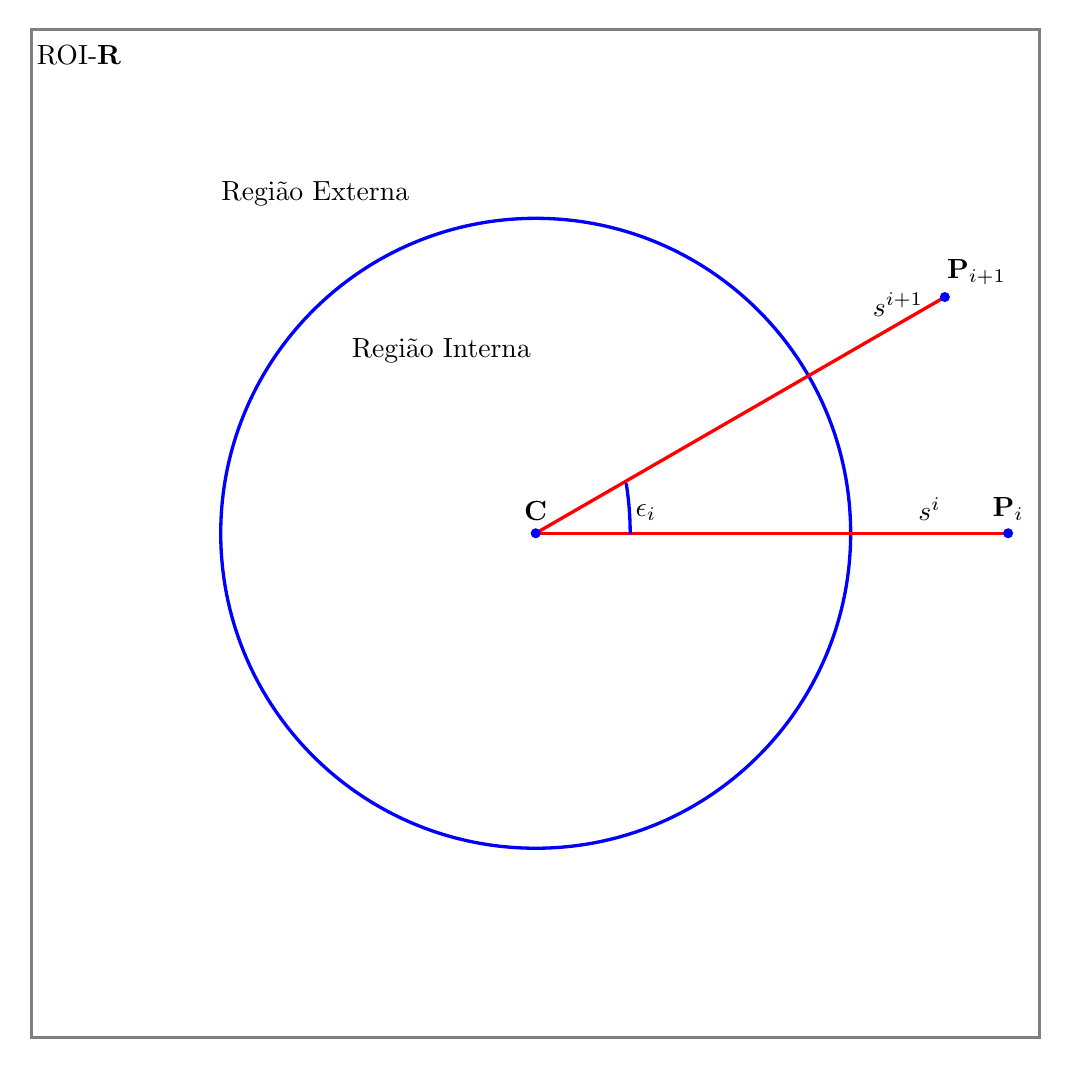
\begin{tikzpicture}[scale=4.0,cap=round,>=latex]
        \draw[blue, very thick] (0cm,0cm) circle(1cm);
        \draw[gray,  very thick] (-1.6,-1.6) rectangle (1.6,1.6);
        \foreach \x in {0,30} {
                \draw[red,  very thick] (0.0cm,0.0cm) -- (\x:1.5cm);
                \filldraw[blue] (\x:1.5cm) circle(0.4pt);
        }
        \draw (1.5cm,0cm) node[above=1pt] {$\mathbf{P}_i$};
        \draw (1.25cm,0cm) node[above=1pt] {$\bm{s}^i$};
        \draw (1.4cm,0.75cm) node[above=1pt] {$\mathbf{P}_{i+1}$};
        \draw (1.15cm,0.65cm) node[above=1pt] {$\bm{s}^{i+1}$};
        \draw (0cm,0cm) node[above=1pt] {$\mathbf{C}$};
        \filldraw[blue] (0cm,0cm) circle(0.4pt);
        \draw (-0.7cm,1cm) node[above=1pt] {Região Externa};
        \draw (-0.3cm,0.5cm) node[above=1pt] {Região Interna};
        \draw (-1.45cm,1.45cm) node[above=1pt] {ROI-$\mathbf{R}$};
        \draw[blue,  very thick] (0.3cm,0) arc (0:9:1);
        \draw (0.35cm,0cm) node[above=1pt] {$\epsilon_i$};
    \end{tikzpicture}
	\caption{Definições para a ROI na imagem PolSAR.}
\label{fig:cap_det_bor_radiais}
\end{figure}
O algoritmo \textit{Bresenham's midpoint line} é usado para definir a radial e extrair informação de cada pixel correspondente da imagem. 
\subsection{Estimativa por máxima verossimilhança}\label{metodo_mle_est_param}
A estimativa por máxima verossimilhança (MLE) estima os parâmetros do modelo estatístico para uma amostra de dados observados.

Suponha $\bm z = (z_1,\dots,z_n)$ um vetor randômico distribuído de acordo com função densidade de probabilidade $f(\bm z,\mathbf{\theta})$ com parâmetros $\mathbf{\theta}=(\theta_1,\dots,\theta_d)^T$ pertencente ao espaço dos parâmetros $\Theta$. Definimos, então a função de verossimilhança 
\begin{equation}\label{eq:funcao_de_verossimilhanca_theta}
   L(\theta;\bm z) = \prod_{k=1}^{n}f(z_k;\theta), 
\end{equation}
e a função log-verossimilhança  
\begin{equation}\label{eq:funcao_de_log_verossimilhanca_theta}
	\mathcal{L}(\theta;\bm z)= \ln L(\theta;\bm z)  = \sum_{k=1}^{n}\ln f(z_k;\theta). \\
\end{equation}

O vetor de parâmetros $\theta$ é estimado pelo vetor $\widehat{\theta}$ tal que $\mathcal{L}(\widehat{\theta};\bm z)\ge \mathcal{L}(\theta;\bm z)$ para todo $\theta$ no espaço dos parâmetros $\Theta$. A estimativa de máxima verossimilhança pode ser representada por 
\begin{equation}\label{eq:max_vetor_log_theta}
    \widehat{\theta}= \text{arg}\,\max\limits_{\theta\in\Theta}\mathcal{L}(\theta;\bm z).\\
\end{equation}
%
\subsection{A máxima verossimilhança usando os parâmetros estimados}\label{sec:sub:mle_param_estimados}
Cada linha radial $\bm z = (z_1,z_2,\dots,z_n)$ é particionada em duas amostras disjuntas na posição $j$,
$$
\bm z = (\underbrace{z_1,z_2,\dots,z_j}_{\bm z_\text{I}}, 
\underbrace{z_{j+1}, z_{j+2},\dots,z_n}_{\bm z_\text{E}}),
$$
para as quais são definidos modelos estatísticos diferentes, um modelo para
$\bm Z_\text{I} \sim W(\Sigma_\text{I},L_\text{I})$, e outro modelo para
$\bm Z_\text{E} \sim W(\Sigma_\text{E},L_\text{E})$.

O método MLE, descrito na seção \eqref{metodo_mle_est_param}, é aplicado nas amostras internas $\bm z_\text{I}$ e externas $\bm z_\text{E}$ para estimar $(\Sigma_\text{I},L_\text{I})$ e $(\Sigma_\text{E},L_\text{E})$ maximizando~\eqref{eq:funcao_de_log_verossimilhanca_theta}, e obtendo $(\widehat{\Sigma}_\text{I}, \widehat{L}_\text{I})$ e $(\widehat{\Sigma}_\text{E}, \widehat{L}_\text{E})$.

A função de verossimilhança é definida no ponto $j$ de acordo com a função
\begin{equation}\label{eq:vero_prod_int_ext}
	L(j)=\prod_{k=1}^{j}f_{\mathbf{Z}}(\bm z_k;\mathbf{\Sigma}_k,L_k) \prod_{k=j+1}^{n}f_{\mathbf{Z}}(\bm z_k;\mathbf{\Sigma}_k,L_k). \\
\end{equation}

Usando propriedades de logaritmos naturais para cada termo do produtório \eqref{eq:vero_prod_int_ext} é definido a função log-verossimilhança total dependendo de $j$,
\begin{equation}\label{eq:log_vero_int_ext}
	\mathcal{L}(j)=\ln L(j)=\sum_{k=1}^{j}\ln f_{\mathbf{Z}}(\bm z_k;\mathbf{\Sigma}_k,L_k)+ \sum_{k=j+1}^{n}\ln f_{\mathbf{Z}}(\bm z_k;\mathbf{\Sigma}_k,L_k).
\end{equation}

O estimador de máxima verossimilhança $\widehat{\jmath}_{ML}$ é uma evidência de borda, pois representa uma aproximação da transição entre regiões, sendo
\begin{equation}\label{eq:max_j_ml}
\begin{array}{rcl}
	\widehat{\jmath}_{ML}&=&\text{arg}\max\limits_{j}\mathcal{L}(j)\\
\end{array}
\end{equation}
a evidência de borda é encontrada aplicando-se o método GenSA~\citep{xgsh}.

\section{O MLE aplicado a pdf $\Gamma$ em cada canal de intensidade}\label{sec:eml_pdf_gamma}
Na função distribuição de densidade univariada gaussiana 
\begin{equation}\label{pdf_gauss_univ}
	f_{Z}(z;\mu,L)=\frac{L^{L}}{\Gamma(L)\mu^{L}} z^{L-1}\exp\left\{-\frac{L}{\mu}z\right\}, \\
\end{equation}
onde, $\mu>0$ e $L>0$, aplicamos o logaritmo natural e suas propriedades,
\begin{equation}\nonumber
\begin{array}{ccl}
	\ln f_{Z}(z;\mu,L)&=&\ln \left(\frac{L^{L}}{\Gamma(L)\mu^{L}} z^{L-1}\exp\left\{-\frac{L}{\mu}z\right\}\right), \\
	                                         &=&\ln\left(\frac{L}{\mu}\right)^L-\ln\Gamma(L)+ \ln z^{L-1} + \ln \exp\left\{-L\frac{z}{\mu}\right\}, \\
%	                                         &=&L\ln\frac{L}{\mu}-\ln\Gamma(L)+(L-1)\ln z - \frac{L}{\mu} z,\\	                                         
\end{array}
\end{equation}
obtendo a função,
\begin{equation}\label{func_log_univ_gaussiana}
	\ln f_{Z}(z;\mu,L)=L\ln\frac{L}{\mu}-\ln\Gamma(L)+(L-1)\ln z - \frac{L}{\mu} z.
\end{equation}

Dado a amostra $\bm z = (z_1,\dots,z_n)$ extraída dos canais de intensidades hh, hv, e vv, é definida a função log-verossimilhança, como  
\begin{equation}\nonumber
\begin{split}
  \mathcal{L}(\bm z;\mu, L)=\ln\prod_{k=1}^{n}f_Z(z_k;\mu,L)\\
  \mathcal{L}(\bm z;\mu, L)=\sum_{k=1}^{n}\ln f_Z(z_k;\mu,L).
 \end{split}
 \end{equation}
 
Com o uso da função logarítmica~\eqref{func_log_univ_gaussiana}, teremos
\begin{equation}\nonumber
\begin{split}
    \mathcal{L}(\bm z;\mu, L)&=\sum_{k=1}^{n}\ln f_Z(z_k;\mu,L)\\
                      &=\sum_{k=1}^{n}\left[L\ln\frac{L}{\mu}-\ln\Gamma(L)+(L-1)\ln z_k - \frac{L}{\mu} z_k\right]\\
                      &=\sum_{k=1}^{n}L\ln\frac{L}{\mu}-\sum_{k=1}^{n}\ln\Gamma(L)+(L-1)\sum_{k=1}^{n}\ln z_k - \frac{L}{\mu}\sum_{k=1}^{n} z_k\\
                      &=L\ln\frac{L}{\mu}\sum_{k=1}^{n}1-\ln\Gamma(L)\sum_{k=1}^{n}1+(L-1)\sum_{k=1}^{n}\ln z_k - \frac{L}{\mu}\sum_{k=1}^{n} z_k\\
                      &=L\ln\frac{L}{\mu}n-\ln\Gamma(L)n+(L-1)\sum_{k=1}^{n}\ln z_k - \frac{L}{\mu}\sum_{k=1}^{n} z_k.\\                
 \end{split}
 \end{equation}

A função log-verossimilhança para a PDF univariada~\eqref{pdf_gauss_univ} pode ser reescrita por
\begin{equation}\nonumber
    \mathcal{L}(\bm z;\mu, L)=n\left[L\ln\frac{L}{\mu}-\ln\Gamma(L)\right]+(L-1)\sum_{k=1}^{n}\ln z_k - \frac{L}{\mu}\sum_{k=1}^{n} z_k,\\                
 \end{equation}
e a sua forma reduzida por 
\begin{equation}
\mathcal{L}(\bm z;\mu, L) = 
n \left[L\ln \frac{L}{\mu} - \ln \Gamma(L)\right]
+L \sum_{k=1}^{n}\ln z_k -\frac{L}{\mu}\sum_{k=1}^{n} z_k.
\label{eq:LogLikelihoodGamma_red}
\end{equation}

A função~\eqref{eq:LogLikelihoodGamma_red} é usada para estimar os parâmetros $(\widehat \mu, \widehat L)$ com o método MLE de $(\mu, L)$ baseado na amostra $\bm z$. O valor máximo da função~\eqref{eq:LogLikelihoodGamma_red} é encontrado com o método BFGS, implementado no pacote \texttt{maxLik} \citep{ht}. Para alcançar uma melhor estabilidade numérica, optou-se por realizar o processo de otimização resolvendo $\nabla\mathcal{L}=\bm 0$. 

De acordo com a seção \eqref{sec:sub:mle_param_estimados} é extraído de cada canal de intensidade da imagem PolSAR uma faixa de dados $\bm z = (z_1,z_2,\dots,z_n)$ de forma que seja particionada em duas amostras, disjuntas na posição $j$:  
$$
\bm z = (\underbrace{z_1,z_2,\dots,z_j}_{\bm z_\text{I}}, 
\underbrace{z_{j+1}, z_{j+2},\dots,z_n}_{\bm z_\text{E}}),
$$
para as quais são definidos modelos estatísticos diferentes, um modelo para
$\bm Z_\text{I} \sim \Gamma(\mu_\text{I},L_\text{I})$, e outro modelo para
$\bm Z_\text{E} \sim \Gamma(\mu_\text{E},L_\text{E})$.

As funções log-verossimilhança reduzidas aplicadas nas amostras internas $\bm z_\text{I}$ e externas $\bm z_\text{E}$ são usadas para estimar os parâmetros $(\mu_\text{I},L_\text{I})$ e $(\mu_\text{E},L_\text{E})$ maximizando~\eqref{eq:LogLikelihoodGamma_red}, e obtendo $(\widehat{\mu}_\text{I}, \widehat{L}_\text{I})$ e $(\widehat{\mu}_\text{E}, \widehat{L}_\text{E})$.


A log-verossimilhança total é definida no ponto $j$ pela seguinte função
\begin{equation}\label{eq:TotalLogLikelihood}
\begin{split}
%\ell(j&;\bm z_\text{I},\bm z_\text{E}) = \\
\ell(j&;\widehat{\mu}_I, \widehat{L}_I,\widehat{\mu}_E, \widehat{L}_E)=\\
&j \big[\widehat{L}_\text{I}\ln (\widehat{L}_\text{I} / \widehat{\mu}_\text{I}) - \ln \Gamma(\widehat{L}_\text{I})\big]
+\widehat{L}_\text{I} \sum_{k=1}^{j}\ln z_k -\frac{\widehat{L}_\text{I}}{\widehat{\mu}_\text{I}}\sum_{k=1}^{j} z_k +\\
&(n-j) \big[\widehat{L}_\text{E}\ln (\widehat{L}_\text{E} / \widehat{\mu}_\text{E}) - \ln \Gamma(\widehat{L}_\text{E})\big]
+\widehat{L}_\text{E} \sum_{k=j+1}^{n}\ln z_k - \frac{\widehat{L}_\text{E}}{\widehat{\mu}_\text{E}}\sum_{k=j+1}^{n} z_k,
\raisetag{2.2em}
\end{split}
\end{equation}
e aplicando o método GenSA~\citep{xgsh} encontramos a evidência de borda
$$
\widehat{\jmath}= \arg\max\limits_{j\in [\min_s,N-\min_s]}\ell(j;\widehat{\mu}_I, \widehat{L}_I,\widehat{\mu}_E, \widehat{L}_E),
$$ 
onde $\min_s$ é uma folga mínima definida empiricamente para as extremidades da amostra. A escolha do número de pixeis da amostra pode variar de acordo com a ROI, com o canal, ou com o tipo de sensor para aquisição de imagem.
